\section{习题 2.7：直纹二次曲面（11 题）}\label{sec:27}
\tip{\textbf{直纹曲面}指曲面可由一族直线完全扫出。单叶双曲面和双曲抛物面都有两族直母线。同族的两条直母线通常异面，而异族的母线可以相交。}
\begin{center}
\begin{tikzpicture}[scale=.8,>=Stealth]
\draw[->] (-.5,0)--(5.5,0) node[right]{$x$};
\draw[->] (2.2,-.5)--(2.2,4.5) node[above]{$z$};
\foreach \a in {0,0.35,...,2.1}{
  \draw[blue!70] plot[domain=-1.7:1.7,samples=15] ({2.2+\x},{2+0.32*(\x*\x-4*(\x-\a)*.35)});
}
\draw[very thick,teal] (.6,3.4)--(4.7,.4);
\node at (8,3.05) {双曲抛物面上的};
\node at (8,2.42) {两族直母线};
\node at (8,1.75) {$z=(x^2-y^2)/2$};
\end{tikzpicture}
\end{center}

\begin{center}
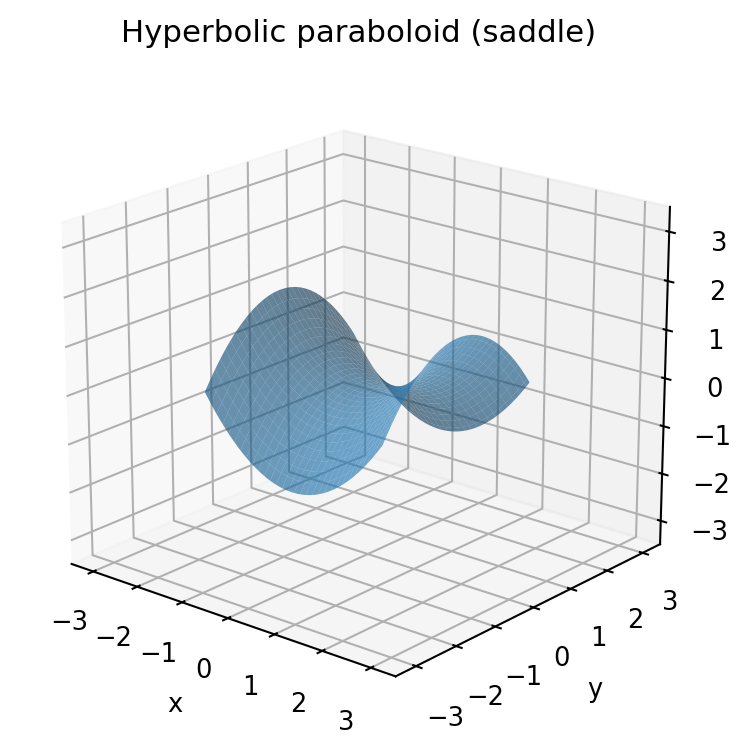
\includegraphics[width=.57\linewidth]{figures/hyperbolic-paraboloid.png}
\figcaptiontxt{双曲抛物面（马鞍面）有两族直母线；看起来弯曲的曲面，仍能由整条直线扫出。}
\end{center}
\Q{1}{求过给定点的两条直母线}
单叶双曲面 $\frac{x^2}{4}+\frac{y^2}{9}-\frac{z^2}{16}=1$，点 $P(2,-3,4)$ 确实在其上。改写为
\[\left(\frac x2+\frac z4\right)\left(\frac x2-\frac z4\right)=\left(1+\frac y3\right)\left(1-\frac y3\right).\]
利用“左右两对因子的比例相等”给出两族平面交线。把 $P$ 代入并整理，得到过 $P$ 的两条直母线：
\ans{$\begin{cases}2x-z=0,\\y+3=0,\end{cases}$ 和 $\begin{cases}4y+3z=0,\\x-2=0.\end{cases}$}
\tip{将两条直线各自代回双曲面，会恒成立；它们都经过 $P$，但方向不同。}

\Q{2}{证明不能有三条直母线同处一张平面}
设某平面 $\pi$ 与非退化直纹二次曲面 $S$ 有三条不同直线作为交集的部分。把 $S$ 的二次方程限制到平面 $\pi$ 上，会成为\emph{平面上的二次多项式}。一个非零二次多项式不能含三条不同直线作为零因子；若它在三条不同直线上恒为零，则限制多项式只能恒等为零，这意味着整张平面包含于 $S$。
但非退化的单叶双曲面或双曲抛物面均不包含完整平面，矛盾。
\ans{故同一张平面最多包含两条曲面直母线，不可能包含三条不同直母线。}

\Q{3}{双曲抛物面上两族正交直母线的交点轨迹}
给定 $x^2-y^2/9=2z$，令
\[u=x+\frac y3,\qquad v=x-\frac y3.\]
方程成为 $uv=2z$。一族母线可写 $u=a,z=av/2$，另一族写 $v=b,z=bu/2$。它们的空间方向向量分别可取
\[d_1=(1,-3,a),\qquad d_2=(1,3,b).\]
两线正交的条件是 $d_1\cdot d_2=1-9+ab=0$，故 $ab=8$。交点同时满足 $u=a,v=b,z=ab/2=4$，即
\ans{$\displaystyle\begin{cases}x^2-\frac{y^2}{9}=8,\\z=4.\end{cases}$ 与书后答案一致。}

\Q{4}{证明双参数线族形成双曲抛物面}
给定不共面的 $u,v,w$ 和点 $A$，令 $\overrightarrow{AA_t}=tw$，直线 $l_t$ 过 $A_t$ 且方向 $v+tu$。其上的点为
\[X=A+tw+s(v+tu)=A+sv+tw+st\,u.\]
以 $A$ 为原点、$v,w,u$ 为一组仿射基，则坐标为
\[(\xi,\eta,\zeta)=(s,t,st),\quad\Longrightarrow\quad \boxed{\zeta=\xi\eta}.\]
经线性代换 $p=(\xi+\eta)/2,q=(\xi-\eta)/2$ 得 $\zeta=p^2-q^2$，这就是标准的双曲抛物面。
\ans{得证。}

\Q{5}{连接两个参数同步点所得的直纹面}
两条给定直线为
\[l_1(t)=(3/2+3t,-1+2t,-t),\quad l_2(t)=(3t,2t,0).\]
连接同一 $t$ 下的两点，并以 $s$ 作为内外分参数：
\[X=(1-s)l_1(t)+s l_2(t).\]
令 $q=1-s$，则
\[x=\frac32q+3t,\quad y=-q+2t,\quad z=-qt.\]
因此
\[-\frac{x^2}{9}+\frac{y^2}{4}=-\left(\frac q2+t\right)^2+\left(-\frac q2+t\right)^2=-2qt=2z.\]
\ans{$\displaystyle-\frac{x^2}{9}+\frac{y^2}{4}=2z$，是双曲抛物面。}

\Q{6}{两异面直线的平面平行横截线族}
设异面线 $l_1=P_1+s u_1,l_2=P_2+t u_2$，要求一条连接两线的横截线平行于给定平面 $\pi$，其法向量为 $n$。条件
\[n\cdot(P_2+t u_2-P_1-s u_1)=0\]
是 $s,t$ 的一次关系。由于题设两线均不平行于 $\pi$，$n\cdot u_1$ 和 $n\cdot u_2$ 均非零，故 $t=\lambda s+\mu$。
横截线上的任一点
\[X=(1-r)(P_1+s u_1)+r(P_2+(\lambda s+\mu)u_2)\]
含有 $r,s,rs$ 三类仿射项，而原两线异面保证它们在一个恰当仿射基下可化为 $w=rs$。\ans{因此横截线族构成一张双曲抛物面。}

\Q{7}{三条两两异面的直线的公共横截线族}
取三条异面直线 $l_i=P_i+t_i u_i$。一条公共横截线在两条线上各有一点 $X(s),Y(t)$，还须经过第三条线的某点。第三个共线条件给出关于 $s,t$ 的一个分式线性关系，所得线族组成一张二次直纹曲面。
根据三条直线的共同方向情况，可分为：
\begin{itemize}
\item 若三条线的方向向量\textbf{共面}，可选一张同时平行三线的平面，横截线族形成双曲抛物面。
\item 若三条线的方向向量\textbf{不共面}，得到单叶双曲面。
\end{itemize}
\ans{这是原书习题 2.7 第 7 题的分类；两种情形都能有两族直母线。}

\Q{8}{过两直线的互相垂直平面，其交线的轨迹}
令 $l_1,l_2$ 为两条给定直线，分别任取过 $l_1,l_2$ 的平面 $\pi_1,\pi_2$，要求 $\pi_1\perp\pi_2$，讨论交线 $\pi_1\cap\pi_2$ 的整体轨迹 $S$。
\begin{enumerate}[label=(\arabic*)]
\item 因任何过 $l_i$ 的平面都包含该直线，所以令点趋向 $l_i$ 上点（或者选择另一张正交平面使它经过该点），可见 $l_1,l_2$ 都落在 $S$ 上。
\item 平面族分别可由单参数 $\lambda,\mu$ 描述，正交条件是两法向量点乘为零，它给出两参数的一次双线性关系。消元后 $S$ 是一张次数不超过二的直纹曲面。
\item 若 $l_1\parallel l_2$，在垂直两线的截面中，要求从两给定截点出发的两条线段互相垂直，交点轨迹为以两截点为直径端点的圆（泰勒斯定理）。随线方向平移得到\textbf{圆柱面}，轴线经过两直线之间的中点并平行于它们，半径为两直线距离的一半。
\item 若 $l_1,l_2$ 相交但不垂直，则 $S$ 的所有母线通过公共点，构成\textbf{非圆锥面}。
\item 若 $l_1\perp l_2$（相交），正交平面族交线退化为\textbf{一对相互垂直的平面}。
\item 若 $l_1,l_2$ 异面且不垂直，则交线族形成\textbf{单叶双曲面}。
\end{enumerate}
\ans{按上述六情形分类，与书后答案一致。}

\Q{9}{与两条直线都相交、又垂直于指定方向的横截线}
$M_1=(1,0,1),u_1=(1,0,1)$；$M_2=(1,1,1),u_2=(0,1,1)$；横截线方向还要求垂直于 $u_3=(1,1,0)$。
取线上点 $P(t)=(1+t,0,1+t)$、$Q(s)=(1,1+s,1+s)$，从 $(Q-P)\cdot u_3=0$ 得 $s=t-1$。所以
\[P=(1+t,0,1+t),\qquad Q=(1,t,t).\]
横截线上的一般点为 $X=(1-r)P+rQ$，即
\[x=1+t-rt,\quad y=rt,\quad z=1+t-r.\]
可消去 $t=x+y-1$、$r=x+y-z$，从 $y=rt$ 得
\[y=(x+y-1)(x+y-z).\]
展开得到
\ans{$x^2+y^2+2xy-xz-yz-x-2y+z=0$，是双曲抛物面。}

\Q{10}{两条直线各过一张互相垂直的平面，求交线族}
给定 $l_1:\frac{x-6}{1}=\frac y2=\frac{z-1}2$ 与 $l_2:\frac x1=\frac{y-8}{2}=\frac{z+4}{-2}$。对各线分别取平面族
\[\pi_1=F_1+\lambda G_1=0,\qquad\pi_2=F_2+\mu G_2=0.\]
令法向量 $n_1(\lambda)\cdot n_2(\mu)=0$；利用这个双线性关系，联立两平面方程并消去 $\lambda,\mu$，可得
\ans{$3y^2-5z^2+4xy-6x-16y+5z+36=0$，是单叶双曲面。}

\Q{11}{与第一条直线正交、与第二条直线共面的直线族}
$l_1$ 过 $P_1=(1,-3,5)$、方向 $u_1=(1,0,1)$；$l_2$ 过 $P_2=(0,2,-1)$、方向 $u_2=(-1,2,0)$。取待求线上一点 $X$、方向 $v$。
其与 $l_1$ 正交且相交的要求，可表示为存在 $t$，使过 $P_1+t u_1$ 的直线满足 $v\cdot u_1=0$；与 $l_2$ 共面的要求为 $\det(X-P_2,u_2,v)=0$。
把与 $l_1$ 相交的点参数以及上述两条件联立，消去直线参数与方向向量，即得
\ans{$2x^2-2z^2+xy+yz+8x+6y+14z+6=0$，是双曲抛物面。}
\clearpage
\section*{整章图形辨析与勘误索引}\addcontentsline{toc}{section}{整章图形辨析与勘误索引}
\begin{enumerate}
\item \textbf{球面：}本章 2.1/2.5 中的球面方程均应由球心、半径、配方得到；若公式退化成点集或空集，不能叫球面。
\item \textbf{仿射系与直角系：}2.2/2.3 的共面、平行判定可以用仿射坐标；2.4 的夹角和距离必须使用直角正交坐标下的欧氏内积。
\item \textbf{消元后的增根：}2.5 锥面、旋转面题常因平方或有理化多出点 / 母线。应保留原参数约束或加以说明。
\item \textbf{原书疑误 A：}2.5 第 5(1) 题，书后椭球分母印为 $5,4,4$；按原题两焦点距离和 $10$，应为 $25,16,16$。
\item \textbf{原书疑误 B：}2.5 第 7(3) 题，书后圆柱面展开式多印常数项 $-5$，所给经过点代入不为零。
\item \textbf{原书疑误 C：}2.6 第 8 题，书后在 $k=a$ 的分类忽略了抛物柱面临界情形。
\item \textbf{直纹二次曲面：}2.7 中 $w=st$ 的双参数构造是证明双曲抛物面有两族直母线的关键。
\end{enumerate}
\tip{\textbf{复习建议：}做曲面题先写清楚\emph{准线、母线、轴线、顶点、截面}各是什么，再用不变量建立方程。做直线和平面题先把所有对象改写成\emph{一点 + 方向/法向量}，最后才考虑行列式运算。}
